\documentclass[a4paper,12pt]{article}
\usepackage[utf8]{inputenc}
\usepackage[T2A]{fontenc}
\usepackage{amsmath}
\usepackage{hyperref}
\hypersetup{colorlinks=true}
\usepackage{colortbl}
\usepackage{graphicx}
\usepackage{float}
\usepackage{gensymb}
%\pagecolor[rgb]{1,1,1}
\pagecolor[rgb]{1,.99,.93}

\usepackage{titlesec}
\newcommand{\sectionbreak}{\clearpage}

\usepackage[symbol]{footmisc}

\usepackage[symbol]{footmisc}

\renewcommand*{\thefootnote}{\fnsymbol{footnote}}

\hypersetup{colorlinks=true, linkcolor=black}

\title{U{\degree}OS blockchain framework}
\author{}

\begin{document}

\clearpage\maketitle
\thispagestyle{empty}
%\maketitle


\clearpage\tableofcontents
\setcounter{page}{1}
%\thispagestyle{empty}


\clearpage
%\setcounter{page}{1}
\begin{abstract}

The concept of a cryptographically protected and distributed transaction ledger has demonstrated its efficiency in a series of projects. Decentralized frameworks based on blockchain technology allow communities to build transparent and reliable peer-to-peer systems that implement economic relationships between the users of the network. Over the recent years a series of consensus protocols were created and utilized in existing blockchain systems \cite{satoshi, dantheman, nem, dbft, poa}. In this paper we introduce the U{\degree}OS blockchain framework and a novel DPoI (Delegated Proof of Importance) consensus algorithm that takes into consideration the value of the social and economic interactions between the members of the network and motivates users to actively contribute to the network growth. Notably, our DPoI metric can be modified to account for a variety of interactions, that arise in a particular network system. DPoI is a high-performance, resource efficient, network-growth inducing algorithm that rewards network participants for the economy enhancing operations in the system. Delegated Proof of Importance is an upgrade to the existing blockchain solutions, that integrates the concepts of the Delegated Proof of Stake (DPoS) and properties of networks. The system protocol is designed in accordance with business and end-user requirements such as privacy, transparency, and smooth volatility, which is achieved due to adaptive emissions proportionate to both network activity growth and the volume of the network itself, according to Metcalfe's law \cite{Metcalfe}. Our U{\degree}OS blockchain framework with the DPoI consensus metric represents a flexible architecture that can be deployed to set up a number of decentralized blockchain-based applications from social networks to service platforms with the direct growing economic value for all users. In this sense, U{\degree}OS is a unique framework that unlike any centralized system can be employed to create highly transparent network-based economies.



\end{abstract}

\section{Introduction}

An unprecedented increase in interest towards blockchain technologies has been observed in the recent years. At this time these technologies were primarily implemented in the form of distributed payment networks \cite{satoshi, stellar, dash, nano} and distributed infrastructure systems \cite{etherium, eos, hyperledger, neo}. These payment networks are decentralized and enable fast low-cost peer-to-peer financial transactions between the users of the system, while infrastructure systems implement smart contracts and decentralized applications (DApps).

The basis of any blockchain system that also determines its technical characteristics is the network consensus algorithm. Namely, consensus algorithm is the mechanism that allows the network nodes to reach the agreement about the contents of the distributed ledger. In this paper we would like to review existing consensus protocol solutions and introduce a novel U{\degree}OS blockchain framework with a corresponding DPoI consensus metric.


\subsection{Previous work}

The problem of distributed consensus for networks with potentially fraudulent participants known as the Byzantine Generals' Problem was stated in 1982, long before the creation of blockchain. \cite{Lamport} Since then an array of different solutions has been developed \cite{Castro}. However, the first solution that did not rely on a trusted third party, was the Proof-of-Work (PoW) algorithm \cite{satoshi}. Despite its advantages, PoW inherently has a number of shortcomings, namely, security \cite{Eyal}, scalability, performance\cite{Croman}, the problem of progressive centralization of the networks around the largest mining pools \cite{Buterin} and, most importantly, the need to use vast volumes of physical resources, such as electricity and computing power to generate blocks. \cite{Bentov}. 

Computing resources needed for block hashing in the current blockchain frameworks, that implement PoW, are tremendous and far exceed the computing power of the world’s greatest supercomputers. Energy use for the block mining is comparable to the power consumption of some countries and it continues to grow \cite{energy}. In 2012, in order to mitigate these shortcomings, the PPCoin, currently  known as PeerCoin, cryptocurrency became the first to utilize an alternative consensus algorithm, Proof-of-Stake (PoS) \cite{Ppcoin}. In PoS consensus networks, the probability of creating a new block depends on the volume of tokens in a participant’s account. Despite significant reduction in resource utilization, PoS turns out to have several drawbacks and in its current state, according to a number of experts, cannot serve as an adequate replacement to PoW \cite{Demeester}, \cite{Poelstra}. One of the major weaknesses of PoS is that it additionally motivates users to concentrate all funds in one place or with one user, which leads to centralization of the network.

The next iteration of PoS was introduced as the Delegated Proof-of-Stake (DPoS) \cite{dantheman}. Here network members are divided into two groups: members, who delegate the authority to create blocks and validate transactions, and validators (block producers). This partition provides better scalability and efficiency. Nevertheless, DPoS still has the problem of motivation for a participant to use their assets actively instead of accumulating them, which has a negative impact on the growth and induces network centralization. 

Yet another consensus metric, the Proof-of-Importance consensus algorithm (PoI), was first introduced in the NEM cryptocurrency \cite{nem}. PoI incentivizes network participants' activity. The major departure from PoS is that block generation probability and reward distribution depends not only on the volume of a user's deposits, but also on the participant's activity rate and reputation. Thus, the algorithm motivates users to be more active by participating in more transactions and contributing to the network development. Despite all its merits, PoI has some shortcomings in efficiency. 


\subsection{Motivation}
As a matter of fact, social and economic interactions are integral components of any network system. Therefore, facilitation of social and economic activities contributes to the network development. We propose here a novel DPoI consensus algorithm that takes into account users' social and financial transactions in order to encourage participation in the network growth and prevent centralization. U{\degree}OS framework with DPoI consensus algorithm allows users to build virtually any network economy system on top of the U{\degree}OS blockchain and assign flexible financial and social activity scores, that reflect the nature of the socio-economic relationships in that particular system. 

DPoI metric provides a mechanism for network growth via emission of tokens for social and economic transactions and also a mechanism of decentralization by accounting for socio-economic activity in the overall importance score. In a summary, DPoI metric supplies three main mechanisms for:
\begin{itemize}
\item network development facilitation via emission allocation for social and economic transactions
\item decentralization via socio-economic importance score calculation
\item deployment of DApps with a wide range of social and economic relationships
\end{itemize}



\section{U{\degree}OS consensus algorithm}

The major goal of U{\degree}OS project is to design a consensus algorithm with an individual influence score metric, that facilitates efficient score redistribution, motivates users to participate actively in the network development and prevents centralization. Modern blockchain solutions have problems with scalability, security and efficiency, and to solve those problems, U{\degree}OS protocol introduces the DPoI (Delegated Proof of Importance) Consensus Algorithm. This consensus algorithm combines the advantages of DPoS and PoI, and delegates validation rights to a limited number of accounts, based not only on the stake value of the protocol members, but also on the their transactional activity, in order to achieve high levels of efficiency and scalability within the network.


The U{\degree}OS consensus algorithm (Delegated Proof-of-Importance, DPoI) is based on the DPoS consensus algorithm \cite{dantheman}. In addition to the individual stake amount, our algorithm also considers incoming financial and social transactions of the user. In the U{\degree}OS Protocol participants have the option of delegating the right to validate blocks to a limited number of accounts through voting, using their personal importance scores, analogous to DPoS. Unlike DPoS, however, DPoI importance score formula is calculated from three components, namely, the stake amount, financial transfer activity and social activity. This framework is highly flexible since the network can collectively choose not only the weight of contribution of each term in the final importance score, but also decide on how to calculate the transfer and social activity scores, given the structure of economic and social interactions in the system. In general, the working principle of the U{\degree}OS Protocol Consensus Algorithm can be explained as follows. 


\subsection{Importance score calculation}

DPoI importance score can be interpreted as an importance rating of an account \textit{i} in the network. It is calculated using the formula below: 

\begin{equation}
	    \label{importance_rating}
	    r_i = (1 - \omega_a - \omega_s) v_i + \omega_a \pi_i + \omega_s \sigma_i
	\end{equation}
where $v_i$ is the stake volume index, $\pi_i$ is the financial activity index, $\sigma_i$ is the social network activity index, and $\omega_a$ and $\omega_s$ are the weight coefficients, that determine the relative significance of each component of the user activity. 

Stake volume index is based on the amount of tokens owned and allocated by the account for the usage of the physical resources (CPU and bandwidth), and represents a balance proportion of the total amount of stake in the system. Thus, an account with non-zero stake balance has non-zero importance score. 

Social and financial activity indices depend on the transactional activity of the account in the most recent time window period, determined by the U{\degree}OS protocol. These indices are calculated using NCDAwareRank algorithm, described in the details in the sections below. We will characterize the main principles of the algorithm, based on the calculation of the financial index $\pi_i$. Later in the separate section we will explain how the algorithm is used to calculate the social activity component $\sigma_i$.  NCDAwareRank gives more preference to the accounts that are tightly integrated in the general network, which helps to make the network resistant to the \emph{splitting account attacks}\footnote{See Appendix 1 Glossary for definition} performed by the botnets with a small number of accounts. Another important feature of the algorithm is the utilization of incoming activity only. This is a PageRank-based paradigm, that ensures a user can obtain the score only from the accounts that refer to it. Such a score is a direct representation of the user's utility for the entire network.

Financial activity index $\pi_i$ is calculated only for the accounts with the stake balance exceeding the $A_0$ threshold. This value is determined by the network. When calculating the account financial activity index only transactions with the amount of tokens higher than $T_0$ are taken into account. That value is also determined by the network. Transactions that do not meet these thresholds are not included. Financial activity index depends on transactions, creation time of which lays in some pre-determined time interval. The duration of this interval is $W$ blocks. Contribution of every transaction decreases exponentially.
%\textcolor{red}{Comment for Lesha Prokopov: do we plan to use the same mechanism for the social activity index}

Noticeably, each network application based on U{\degree}OS framework can define their unique set of financial and social transactions that are included in the calculation of the corresponding financial and social index scores. These applications can be deployed as DApps (distributed applications) and may implement a wide range of economic and/or social systems, such as service platforms, knowledge networks, digital content copyright systems, libraries, public records, online markets etc. Unlike centralized versions of such services, U{\degree}OS DApps would preserve the important properties of blockchain systems, particularly, decentralization, record immutability, and transparency.






\subsubsection{Financial activity score calculation}
The vector of financial indices $\boldsymbol{\pi^{(j)}}$, where $j$ is the indicator of the iteration in the algorithm, is calculated according to the NCDAwareRank, following the recurrent relation: 

\begin{equation}
	    \label{recurrent_formula_for_ncdawarerank}
	    \boldsymbol{\pi}^{(j+1)} = ( \alpha \boldsymbol{O} + \beta \boldsymbol{M} + ( 1 - \alpha - \beta ) \boldsymbol{E} ) \boldsymbol{\pi}^{(j)}
	\end{equation}

Here $\boldsymbol{\pi^{(j)}}$ is a vector of the financial activity score index values. The vector is standardized, i.e. the sum of its elements is 1. $\boldsymbol{O}$ is the outlink matrix, $\boldsymbol{M}$ is the interlevel proximity matrix. See the definitions of the matrices below. Coefficients $\alpha$ and $\beta$ are the weights that determine contributions of the matrices $\boldsymbol{O}$ and $\boldsymbol{M}$. Their sum must be less than 1. $\boldsymbol{E}$ is the teleportation matrix, added to ensure that the series is convergent. This matrix is defined as follows:
$$
\boldsymbol{E}=\frac{1}{N}\boldsymbol{\hat{E}}
$$
where \textit{N} is the number of the accounts and $\boldsymbol{\hat{E}}$ is the matrix in which all the elements are equal to 1, the calculation continues until for some $j$ the following condition is fulfilled: 



$$
\lVert \boldsymbol{\pi}^{(j+1)}-\boldsymbol{\pi}^{(j)} \rVert <\delta
$$

Here $\lVert \cdot \rVert$ is the vector norm defined as the sum of its elements, $\delta$ is the predetermined calculation accuracy. As an initial approximation, a vector $\boldsymbol{\pi^{(0)}}$ with all the elements equal to $\frac{1}{N}$ can be used.



\paragraph{Outlink matrix calculation:}
The outlink matrix $\boldsymbol{O}$ is calculated as follows. First, the weight matrix is calculated:



$$
w_{ij}=\sum_{k|j \to i, {h_k \ge H_0} \land {h_k \le H_0+W}} \theta ( a_k - T_0 ) \theta ( s_i - A_0 ) \theta ( s_j - A_0 ) a_k \exp{(lnK [\frac{h_k}{D}])}
$$

where $a_k$ is the token sum of transaction \textit{k}, $h_k$ is the $k$-th transaction depth, i.e. the block order number from the current point, also known as a block height,  $K$ and $D$ are transaction contribution decrease parameters, that define how much the contribution of each transaction decreases over time, $\theta$ is the standard Heaviside step function, and $[ \cdot ]$ is a standard floor function. According to the formula, transaction contribution decreases with the rate $K$ over every $D$ number of blocks, created after this given transaction. The sum is taken over all the transactions of a deposit from the account \textit{i} to the account \textit{j}, depth of which lays between $H_0$ and $H_0+W$. $H_0$ and $W$ are the parameters, which values are currently equal to $H_0=0$ and $W=17280000$ blocks. In this setting only, the transactions from the time gap, duration of which is $W$ blocks, contribute to the financial activity index calculation. Thus, we obtain the coefficient of the incoming financial activity from the user $j$ to the user $i$ as follows:

$$
\hat{o}_{ij} = \begin{cases}
 w_{ji}-w_{ij}
 & \text{if $w_{ji}-w_{ij} > 0$,}\\
 0 & \text{otherwise.}
\end{cases}
$$

After that the matrix, that was obtained, is standardized so that the sum of the elements in every column is equal to 1.


$$
o_{ij} = \begin{cases}
 \frac{\hat{o}_{ij}} {\sum\limits_{k} \hat{o}_{kj}}
 & \text{if $\sum\limits_{k} \hat{o}_{kj}> 0$,}\\
 0 & \text{otherwise}
\end{cases} 
$$
Outlink matrix $\boldsymbol{O}$ captures the structure of incoming financial transactions in the network graph.

\paragraph{Interlevel proximity matrix calculation:}
Let $\Omega$ be the set of all the accounts used for the financial activity index calculation. $\Omega$ is further divided into disjoint subsets $A_i$, called NCD (Nearly-Completely Departed) blocks. These blocks are obtained using the SCAN algorithm, described below. For the given account $u$, $G_u$ is the set of all the accounts, for which the according member of the outlink matrix $o_{vu}$ is greater than zero. Then the set $\chi_u$ of proximal accounts of $u$ is obtained as: 



$$
\chi_u = \bigcup_{v \in \{u\} \cup G_u} A_{(v)}
$$

The interlevel proximity matrix is defined as follows:



$$
M_{vu}=\begin{cases}
 \frac{1}{N_u |A_{(v)}|}
 & \text{if $v \in \chi_u$ ,}\\
 0 & \text{otherwise.}
\end{cases}
$$

where $N_u$ is the number of NCD-blocks in $\chi_u$. Interlevel proximity matrix $M$ represents the structure of connectedness within the network.



\paragraph{SCAN-based network partitioning:}
SCAN algorithm is used to partition network graph into clusters and to prevent activity imitation or fraud between several affiliated accounts \cite{SCAN}. An indirected graph $G = \{V, E\}$ has every vertex, representing a user, and every edge, representing a non-zero element of the outlink matrix. The structure of the vertex $v$ is the set of all the adjacent vertices:


$$
\Gamma(v)=\{w \in V|(v,w) \in E\} \cup \{v\}
$$

The structural similarity of two vertices can be defined as follows:



$$
\sigma(v,w)=\frac{ |\Gamma(v) \cap \Gamma(w)|}{\sqrt{|\Gamma(v)||\Gamma(w)|}}
$$

The vertex $\varepsilon$-neighborhood is a set of vertices for which


$$
N_{\varepsilon}(v) = \{ w \in \Gamma(v) | \sigma(v,w) \ge \varepsilon \}
$$

The \textit{CORE} is a vertex for which the number of elements in the $\varepsilon$-neighborhood is more than $\mu$.

$$
CORE_{\varepsilon,\mu}(v) \Leftrightarrow |N_{\varepsilon} (v)| \ge \mu
$$

Vertex $w$ is directly structurally reachable from vertex $v$ if



$$
DirREACH(v,w) \Leftrightarrow CORE_{\varepsilon,\mu}(v) \vee w \in N_{\varepsilon}(v)
$$

Vertex $w$ is structurally reachable from vertex $v$ if


$$
REACH(v,w) \Leftrightarrow \exists v_1,...,v_n \in V \text{: } \forall i \in \{1,...n-1\} \text{: } DirREACH(v_i,v_{i+1})
$$

Vertex $v$ is structurally connected with vertex $w$ if



$$
CONNECT(v,w) \Leftrightarrow \exists u \in V\text{: } REACH(u,v) \vee REACH(u,w)
$$

A cluster is a subset of vertices structurally connected to each other. It is possible to show that every vertex can only belong to one cluster. A vertex can also belong to no cluster; in this case it can either be a hub if there are vertices belonging to two different clusters in its environment, otherwise it is an independent vertex.


%\begin{figure}[h]
 %     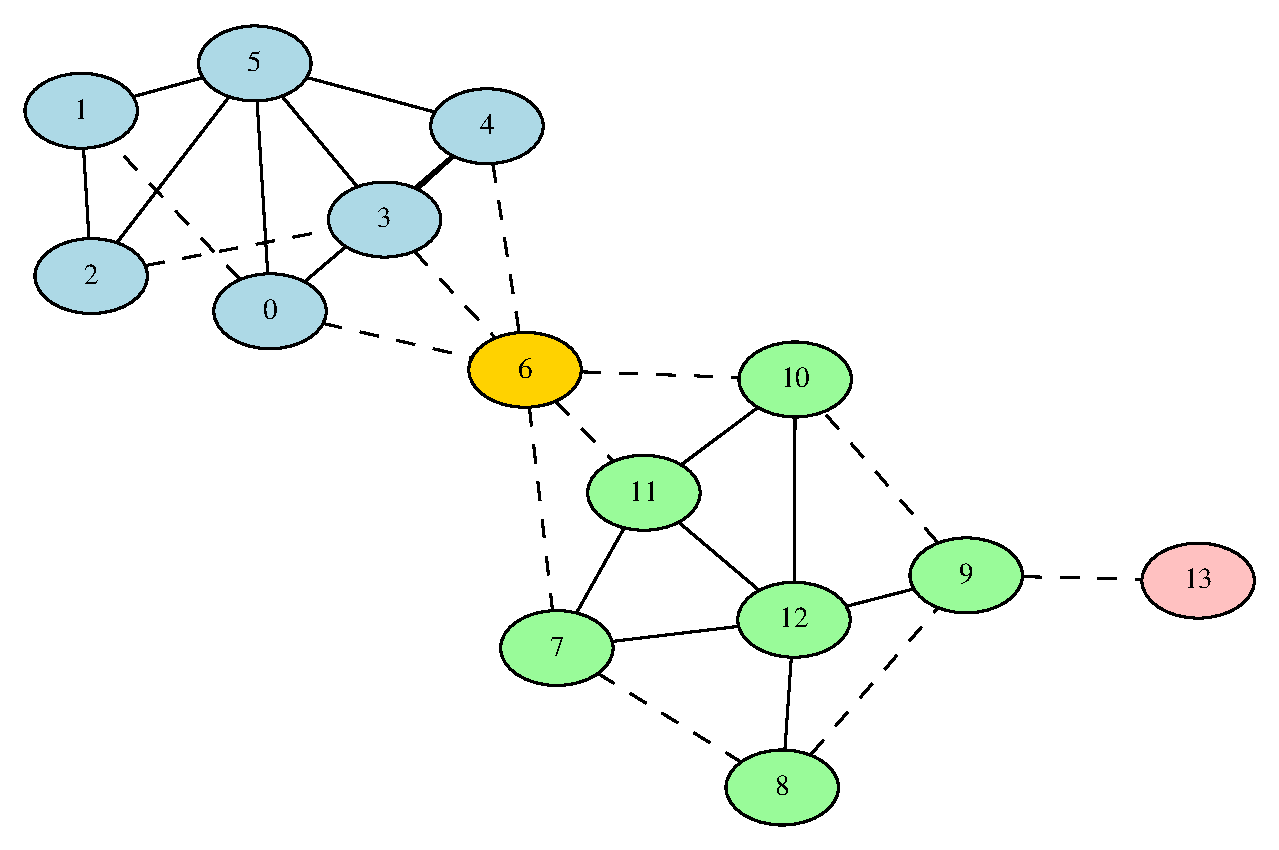
\includegraphics[width=1\linewidth]{pictures/clustering_example.eps}
   %   \caption{SCAN algorythm applying example. Parameters $\varepsilon=0.7$ and $\mu=4$ were used.}
     % \label{fig:sigmoida}
%\end{figure}


\subsubsection{Social activity score calculation}

U{\degree}OS blockchain interacts with a variety of DApps and registers a defined set of social transactions in the network. Each account issues outgoing activity and receives input from other users. Together these connections form a graph with directed edges between the account nodes. Social rates, obtained by the accounts, depend on the amount of the incoming social activity, which constitutes the utility of the user to the whole network. We denote this rate as the social network activity index. It contributes to the general importance rate, defined by the formula (\ref{importance_rating}).  

Social index calculation is based on several pieces of data. First, we define the matrix $\boldsymbol{V}$, that contains the information about the upvote transactions, with elements:
	
	$$	
	V_{ik} = \begin{cases}
	 e^{[h_\alpha/D]ln K}
	 & \text{if the account $k$ upvoted the content $i$ at the height $h_\alpha$,}\\
	 0 & \text{otherwise.}
	\end{cases}
	$$
	
	where $h_\alpha$ is the $\alpha$-th transactional height within the window with a fixed length $W$, i.e. the block height from the current time point.
	
	Second, the matrix $\boldsymbol{P}$ contains the information about the content owners:
	$$
	P_{ik} = \begin{cases}
	 1
	 & \text{if the content $k$ belongs to the account $i$,}\\
	 0 & \text{otherwise.}
	\end{cases}
	$$
	
	Third, the matrix $\boldsymbol{R}$ contains the information about the reposts:
	$$
	R_{ik} = \begin{cases}
	 1 & \text{if the content $i$ is a repost of the account $k$,}\\
	 -1 & \text{if $i=k$ and the content $i$ is a repost,}\\
	 0 & \text{otherwise.}
	\end{cases}
	$$
	
	Given these matrices, we attain the matrix $\boldsymbol{V'}$:
	$$
\boldsymbol{V'} = ( \boldsymbol{I} + \boldsymbol{R} ) \boldsymbol{V}
$$
	%$$
	
	and the intermediate matrix $\boldsymbol{\hat{U}}$, with elements:
	$$
	\hat{U}_{ik} = max_n(P_{in} V'_{nk})
	$$
	As it is characterized by the matrix $\boldsymbol{V}$, weights of the individual transactions $V_{ik}$ decay with time. Some accounts, however, might not have any incoming activity for a period of time, longer than the window $W$. This results in the columns with zero elements in the matrix $\boldsymbol{V}$. Such condition violates the matrix stochasticity, that is necessary for the convergence of the iterative PageRank procedure. 
	
	There are several ways to resolve the issue. First solution is to fill the empty columns with equal values, while second option is to add a value of $1$'s to the diagonal elements of the matrix. Nevertheless, these solutions have notable drawbacks. In a former case, we would diffuse the account rates, such that the difference between the rates of active and inactive accounts becomes insignificant. In a later case, own activity of the account would result in the user rate decrease, contrary to their interest.
	
	In order to provide effective decaying weights and preserve the matrix stochasticity, we add a special hidden account $h$, which accepts upvotes from every account. For this account:
	
	$$
	\forall i \ne h \text{: } \hat{U}_{hi} = 1,
	\forall i  \text{: } \hat{U}_{ih} = 0
	$$
	
	And after standardization:
	$$
U_{ik} = \begin{cases}
 \frac{\hat{U}_{ik}} {\sum_n{\hat{U}_{nk}}} & \text{if $\sum_n{\hat{U}_{nk}}>0$} \\
 0 & \text{otherwise.}
\end{cases}
$$

	Unlike solutions, outlined previously, our answer does not have the mentioned drawbacks. Conversely, it presents several advantages. First of them is that we can now measure the activity of the network with regards to a fixed standard. We can monitor what proportion of the overall network rate is received by the hidden account, which indicates the rate of activity in the network — the higher is the rate of this account, the lower is the network activity. Second, now we have a standard, relative to which we can observe the weights decay. Since transactions towards the hidden account happen regularly, the relative balance between the social index scores of the hidden account and other nodes demonstrates the level of score decay.
	
	Besides above mentioned matrices, calculations of social index scores are based on the stack vector $\boldsymbol{s}$ and a validity weight vector $\boldsymbol{v}$, containing the validity values for every account. These values originate from the trust relationships on the network, and are described in details in the section 2.1.3 below.
	
	Based on these data structures, we can calculate social activity vectors for the accounts $\boldsymbol{\sigma^a}$ and for the content $\boldsymbol{\sigma^c}$. These vectors are standardized to 1:
	
	$$
	\sum_i{\sigma^a_i} = 1, \sum_i{\sigma^c_i} = 1
	$$
		
	
	We calculate the values $\boldsymbol{\sigma^a}$ with a modified PageRank routine:
	
	\begin{equation}
	\label{social_score_pgrank}
	\boldsymbol{\hat{\sigma}^a}^{(n+1)} = (\alpha \boldsymbol{U} + (1 - \alpha) \boldsymbol{T})\boldsymbol{ \hat{\sigma}^a}^{(n)}
	\end{equation}
	
	where the teleportation matrix $\boldsymbol{T}$ contains the information about the initial weights of the accounts
	
	\begin{equation}
	    \label{teleportation_matrix_definition}
        \boldsymbol{T} = ((1 - \beta - \gamma) \boldsymbol{e} + \beta \boldsymbol{v} + \gamma \boldsymbol{s}) \boldsymbol{e}^T
	\end{equation}
	
	Here $\beta$ and $\gamma$ are the coefficients with values between 0 and 1, $\boldsymbol{e}$ is а unit vector, $\boldsymbol{s}$ is the stack vector, and $\boldsymbol{v}$ is the validity vector. Utilization of a validity vector serves as the modification of a classical PageRank algorithm.
	
	We should subtract the contribution of a stack from the rating vector, because social index of an account should not depend on its own stack:
	
	$$
	\boldsymbol{\dot{\sigma}^a} = \frac{1}{1 - (1-\alpha) \gamma}(\boldsymbol{\hat{\sigma}^a} - (1 - \alpha) \gamma \boldsymbol{s})
	$$
	
	Finally, we must remove the rating vector of the hidden account. This operation changes norm of the rating vector, so we must standardize it to 1:
	
	$$
	\sigma^a_i = \frac{\dot{\sigma}^a_i}{\sum_{j \ne h} \dot{\sigma}^a_j}, i \ne h
	$$
	
	
	Based on $\boldsymbol{\sigma^a}$, we obtain values in $\boldsymbol{\sigma^c}$:
	
	$$
	\boldsymbol{\sigma^c} = \boldsymbol{V'}\boldsymbol{\sigma^a}
	$$
	
\subsubsection{Validity trust network}

	Normally, PageRank starts the calculation with the vector of equaly distributed weights, but in our algorithm for social index rate calculation, we modify this vector to integrate the system of trusts in our calculations. This is our innovation, that helps further protect the network from the botnets. Trusts are assigned by the members of the network to other members in a manual fashion and serve as a validation of their accounts. The user transmits trust proportionally to their stack amount. Such a condition ensures that a high level of trust is provided only by the meaningful users in the network. The higher is the level of overall trust that account obtains the higher is potentially the social index rate, they might receive.
	
The validity vector $\boldsymbol{v}$ is used in the formula (\ref{teleportation_matrix_definition}). As mentioned before, it is invented in order to implement additional botnet attack protection and is calculated using the PageRank algorithm.
	
	\begin{equation}
	\label{trust_pagerank}
	\boldsymbol{\hat{v}}^{n+1} = (\alpha O_T+(1-\alpha)T_T) \boldsymbol{\hat{v}}^{n}
	\end{equation}
	
	Here $O_T$ is outlink matrix, that is based on the \textit{trust} relations, $T_T$ is the teleportation matrix:
	
	$$
        \boldsymbol{T_T} = ((1 - \lambda) \boldsymbol{e} + \lambda \boldsymbol{s}) \boldsymbol{e}^T
	$$
	Validity trust scores, obtained with the PageRank algorithm in (\ref{trust_pagerank}), are turned into binary values, using the Heaviside step function $\theta$:
	$$
	\dot{v}_i = \theta({\hat{v}_i}-1/N)
	$$
and standardized towards a sum of $1$:
	$$
	v_i = \frac{\dot{v}_i}{\sum_k{\dot{v}_k}}
	$$
	These scores are later used in (\ref{social_score_pgrank}).
\subsection{Importance score usage: network governance and emission}

Importance index $r_i$ in the framework is used for two major purposes:
\begin{itemize}
\item  network governance through voting for validators (block producers), \emph{calculator nodes}\footnote{See Appendix 1 Glossary for definition} and change of the algorithm parameters
\item emission calculation for each user \textit{i}
\end{itemize}

 %user rankings is not a part of the algorithm

First, it defines the amount of new tokens received by the account in case when the emission is positive.  See section 3 for details.

Second, importance index defines the relative weight of the account during the voting for producers and for the \emph{calculator nodes}\footnote{See Appendix 1 Glossary for definition}. A single user can offer their candidacy for both groups. Voting allows the delegation of certain powers within the system to a limited number of the validation accounts. Producers, that own nodes which produce and verify blocks, as well as the \emph{calculator node}\footnote{See Appendix 1 Glossary for definition} owners, are selected by voting by other members of the network. Candidates nominate themselves for a desired position and voting can be performed by other users at any time. Changes are recorded within a short period, according to the protocol routine.

Change of the blockchain algorithm parameters and the block validation procedure is performed using voting as well. Here users delegate these decisions to the \emph{calculator nodes}\footnote{See Appendix 1 Glossary for definition}.



%\textcolor{red}{Comment: we might want to include here the details of implementation of the changes in the blockchain algorithm, achieved by the consensus on the \emph{calculator nodes}\footnote{See Appendix 1 Glossary for definition}, and on the block production, achieved by consensus among validators.}


\subsection{Key features of the algorithm: resistance to attacks}

Following mitigations are used in the project in order to reduce the risk of attacks:

\begin{itemize}
  \item Only incoming transfers contribute to the importance index, which makes obtaining score from the existing accounts more difficult.
  \item There are stake thresholds for accounts, participating in the importance index calculation, and also the amount thresholds for transfers, which makes attacks more expensive for the attackers.
  \item NCDAwareRank algorithm makes the system more resistant to \emph{splitting account attacks}\footnote{See Appendix 1 Glossary for definition}. This algorithm gives preference to accounts, tightly integrated into the common network.
  \item Coefficients $\omega_a$ and $\omega_s$ have relatively small values, this makes contribution of activity index and social index to total importance index significantly smaller than the stake contribution.
  \item Usage of the decaying weights makes effect of any fraud activity temporary. 
\end{itemize}


\section{Emission}

\subsection{U{\degree}OS token utilization}

U{\degree}OS tokens constitute the core of our crypto-economy. They are used in the system in several ways:

\begin{itemize}
\item to allocate CPU and bandwidth resources, using staked token amounts. Only core U{\degree}OS tokens can be used for CPU and bandwidth resource allocation.
\item to purchase other resources, such as RAM, and perform other forms of financial transfers via smart contracts using unstaked tokens. Potentially, many types of tokens can be used for these activities.
\item to vote for block producers and \emph{calculator nodes}\footnote{See Appendix 1 Glossary for definition}. The amount of staked tokens, owned by the account, contributes to the user's importance during the voting process.
\item to increase the importance score and receive the dynamic emission. Amount of tokens staked by the account directly influences the importance received by the user and the amount of dynamic emission.
\end{itemize}

Thus, staked core tokens are used for the resource allocation and play an important part in emission and importance calculation, while unstaked tokens can be used in direct transfers. 
%The amount of transactions processed directly depends on the available computing power provided by network members. To allocate the resources efficiently and to avoid spam attacks, a fee in the protocol core cryptographic token is levied on the operations within the U{\degree}OS network. The protocol allows a user to make token transfer transactions between the network members and launch system smart contracts, e.g. multi-signature, account registration, user tokens creation and so on.

Emission amount at launch constitutes one billion of protocol tokens, distributed to the original network accounts to start the protocol. The U{\degree}OS project implements adaptive emission. The emission volume is calculated regularly, in a certain time interval, $t_0, t_1, ... t_i$, where $t_{i+1} = t_i + T$. The volume of emission depends on the network activity growth in the preceding time period $T$.


\subsection{Network activity calculation for a period of time}

In order to calculate the emission, we first need to calculate the network activity for the unit time period $T$, defined by the U{\degree}OS protocol. To begin, we calculate the matrix of weights, according to the formula:



$$
w_{ij}(t_n)=\sum_{k|j \to i, t_k \in [t_{n-1}, t_n]}a_k
$$

Here $a_k$  is the sum amount in k-th transaction, $t_k$ is the time at which k-th transaction was created. Summation is performed for all the transactions transferring any amount from account $j$ to account $i$ and created at the time frame from $t_{n-1}$ to $t_n$. 

In fact, each matrix element $w_{ij}$ represents a weight of connection between account $i$ and account $j$ in a given time frame. Next we need to calculate the matrix of connections $l$: 



$$
l_{ij}(t_n) = \begin{cases}
 1
 & \text{if $w_{ji}(t_n)-w_{ij}(t_n) > 0$,}\\
 0 & \text{otherwise.}
\end{cases}
$$

We calculate the activity in a given time frame as:



$$
A(t_n) = \sum_{i,j} l_{ij}(t_n)
$$

In this way, activity is calculated as a number of connections between active accounts in a set timeframe. 



\subsection{Emission value calculation}

Target emission value $E_T$ depends on the network activity growth. It defines the upper bound of the aggregate amount of the emission, that is achievable with the following activity value $A$:



$$
\Delta A(t_n) = A(t_n) - A_{max}(t_{n-1})
$$

$$
E_T(t_n) = \begin{cases}
 E_T(t_{n-1}) + K_E \Delta A(t_n),
 & \text{when $\Delta A(t_n) > 0$,}\\
 E_T(t_{n-1}) & \text{otherwise}
\end{cases}
$$

Here $K_E$ is a coefficient that defines the maximum value of the emission with the activity increased by 1. $A_{max}(t_{n-1})$ is the previous maximum value since the system launch:



$$
    A_{max}(t_{n-1}) = max \Big ( A(t_i), t_i \in [t_0, t_{n-1}] \Big )
$$

Emission value, which is issued at a certain time $t_n$, is defined by the formula:



$$
    E(t_n) = \lambda S(t_{n-1}) f \Big( \kappa \frac {E_T(t_n) - E_S(t_{n-1})}{\lambda S(t_{n-1})} \Big)
$$

Here $\lambda$ is the marginal growth of the token amount in the system S per one emission. It is defined through $L$, which specifies the marginal growth $S$ in a year, expressed as a percentage:



$$
    \lambda = (1 + \frac{L}{100})^{1/N}-1
$$

Here $N$ is the number of emission issues per year.



$f(x)$ - is a sigmoidal function. In the present implementation of the algorithm a hyperbolic tangent is used as this function. 


$\kappa$ is a coefficient between 0 and 1 and it defines the speed at which a full emission approaches the target emission $E_T$ if the activity level remains the same over the long term.



Initial values of both $E_T$ and $E_S$ are zero:



$$
E_T(t_0)=0, E_S(t_0)=0
$$


%\begin{figure}[h]
 %     \includegraphics[width=1\linewidth]{pictures/sigmoida.eps}
  %    \caption{Sigmoidal function}
   %   \label{fig:sigmoida}
%\end{figure}

Dynamic emission allocated to a user for their social and financial activities motivates the user to participate in the network development, thus, helping to achieve the overall network growth.

%\section{Network governance}
%Network governances encompasses several major activities:
%
%\begin{itemize}
%\item choice of block producers and importance calculator nodes 
%\item change of blockchain algorithm parameters and block validation procedure
%\item \textcolor{red}{Comment: anything else?}
%
%\end{itemize}
%Above mentioned network governance activities are performed by the network in a collective manner through voting procedures. Importance score of each user represents the weight of their vote.

\section{U{\degree}OS framework architecture}
In this section we outline the general architecture of the U{\degree}OS blockchain.\footnote{Detailed documentation is located at the U{\degree}OS GitHub and at the EOS.io website: https://developers.eos.io}We have several types of nodes in the system, connected via the peer-to-peer protocol, namely, \emph{api}, \emph{block producer}, \emph{calculator}, and \emph{seed} nodes. Nodes that have a connection between each other are called \emph{peer} nodes. Nodes can be accessed by the owner alone or by any user via \emph{private} or \emph{public} APIs, respectively. Every node, irregardless of their type, performs the following activities:
\begin{itemize}
\item[•] synchronizes and distributes pending transactions into new blocks and new blocks between the peer nodes via peer-to-peer connection
\item[•] communicates with the other programs and receives the information about the state of the blockchain (accounts, token sums, list of block producers, voting results, smart contracts, data tables, transaction blocks, and others) via private and public APIs
\end{itemize}

The node types are briefly defined as follows:
\begin{itemize}
\item \emph{Block producer node} -- owned by the block producer, issues blocks according to the schedule and distributes them among the peer nodes
\item \emph{Calculator node} -- calculates user importance scores, based on social and financial transactions from irreversible blocks, and saves the results to the blockchain
\item \emph{Seed node} -- a node, that has a public peer-to-peer connection, it is used by the new network participants, when they join the network
\item \emph{API node --} a node with a public API
%\item \emph{MongoDB node --}
%\item IPFS nodes
\end{itemize}


\addcontentsline{toc}{section}{Appendix 1 Glossary}

\section*{Appendix 1 Glossary}
\textbf{U{\degree}OS consensus algorithm (Delegated Proof-of-Importance, DPoI)}

The consensus algorithm, which is based on a calculation of the importance index of an account, which in turn depends on Stake Volume Index and Activity index

\textbf{Importance index}

The importance index of an account is calculated as a function of Stake Volume Index and Activity index

\textbf{Account}

An entity represented by a tuple of pairs of keys (public + private), which is registered in a blockchain by an individual.

\textbf{Block Producers}

Accounts with the right to verify blocks. They must have a node.

\textbf{Node}

A P2P network node, which performs all the calculations in blockchain. A node belonging to a producer account (producer node), produces blocks.

\textbf{Calculator node} 

A node that performs importance score calculation and distributes calculated scores back to the network

\textbf{Splitting account attack} 

An attack performed by a network of many accounts. The goal of the attacker is to receive a maximal total importance rate while utilizing minimal resources
\addcontentsline{toc}{section}{References}
\begin{thebibliography}{99}
 \bibitem{Metcalfe} Metcalfe, B. (2013). Metcalfe's law after 40 years of ethernet. Computer, 46(12), 26-31. URL: http://ieeexplore.ieee.org/abstract/document/6636305/
 \bibitem{Lamport} Lamport, L., Shostak, R., Pease, M. (1982). The Byzantine generals problem. ACM Transactions on Programming Languages and Systems (TOPLAS), 4(3), 382-401. URL: https://www.microsoft.com/en-us/research/uploads/prod/2016/12/The-Byzantine-Generals-Problem.pdf
 \bibitem{Castro} Castro, M., Liskov, B. (2002). Practical Byzantine fault tolerance and proactive recovery. ACM Transactions on Computer Systems (TOCS), 20(4), 398-461. URL: https://dl.acm.org/citation.cfm?doid=571637.571640
 \bibitem{satoshi} Nakamoto, S. (2008). Bitcoin: A peer-to-peer electronic cash system. URL: https://bitcoin.org/bitcoin.pdf
 \bibitem{Croman} Croman, K. et al. (2016). On scaling decentralized blockchains. In International Conference on Financial Cryptography and Data Security (pp. 106-125). Springer, Berlin, Heidelberg. URL: http://www.comp.nus.edu.sg/~prateeks/papers/Bitcoin-scaling.pdf
 \bibitem{Eyal} Eyal, I., Sirer, E. G. (2014). Majority is not enough: Bitcoin mining is vulnerable. In International conference on financial cryptography and data security (pp. 436-454). Springer, Berlin, Heidelberg. URL: https://arxiv.org/pdf/1311.0243.pdf
 \bibitem{energy} Bitcoin Energy Consumption Index. digiconomist.net. URL: https://digiconomist.net/bitcoin-energy-consumption
 \bibitem{Buterin} Buterin, V. (2014). Mining Pool Centralization at Crisis Levels. URL: https://bitcoinmagazine.com/articles/mining-pool-centralization-crisis-levels-1389302892/
 \bibitem{Bentov} Bentov, I., Gabizon, A., Mizrahi, A. (2016). Cryptocurrencies without proof of work. In International Conference on Financial Cryptography and Data Security (pp. 142-157). Springer, Berlin, Heidelberg. URL: https://link.springer.com/chapter/10.1007/978-3-662-53357-4\_10/
 \bibitem{Ppcoin} King, S., Nadal, S. (2012). Ppcoin: Peer-to-peer crypto-currency with proof-of-stake. URL: https://peercoin.net/assets/paper/peercoin-paper.pdf
 \bibitem{Demeester} Demeester, T. (2017). Critique of Buterin’s A Proof of Stake Design Philosophy. URL: https://medium.com/@tuurdemeester/critique-of-buterins-a-proof-of-stake-design-philosophy-49fc9ebb36c6
 \bibitem{Poelstra} Poelstra, A. (2014). Distributed consensus from proof of stake is impossible. URL: https://download.wpsoftware.net/bitcoin/old-pos.pdf
 \bibitem{dantheman} Dantheman. (2017). DPOS Consensus Algorithm - The Missing White Paper. URL: https://steemit.com/dpos/@dantheman/dpos-consensus-algorithm-this-missing-white-paper
 \bibitem{nem} NEM Technical Reference. Version 1.2.1. February 23, 2018 URL: https://nem.io/wp-content/themes/nem/files/NEM\_techRef.pdf
\bibitem{SCAN} Xiaowei Xu et al. (2007). SCAN: A Structural Clustering Algorithm for Networks. URL: http://www1.se.cuhk.edu.hk/~hcheng/seg5010/slides/p824-xu.pdf
\bibitem{dbft} Zhang E., A Byzantine Fault Tolerance Algorithm for Blockchain. URL: https://docs.neo.org/en-us/basic/consensus/whitepaper.html
\bibitem{poa} VIVA White paper (2017). URL: https://s3.amazonaws.com/vivacoin/viva-white-paper-v-2-0.pdf
\bibitem{stellar} David Mazieres, (2016), The Stellar Consensus Protocol: A Federated Model for Internet-level Consensus. URL: https://www.stellar.org/papers/stellar-consensus-protocol.pdf
\bibitem{dash} Evan Duffield and Daniel Diaz, (2018), Dash: A Payments-Focused Cryptocurrency. URL: https://github.com/dashpay/dash/wiki/Whitepaper
\bibitem{nano} Colin LeMahieu, (2015), Nano: A Feeless Distributed Cryptocurrency Network. URL: https://nano.org/en/whitepaper
\bibitem{etherium} A Next-Generation Smart Contract and Decentralized Application Platform (2018). URL: https://github.com/ethereum/wiki/wiki/White-Paper
\bibitem{eos} EOS.IO Technical White Paper v2 (2018). URL: https://github.com/EOSIO/Documentation/blob/master/TechnicalWhitePaper.md
\bibitem{hyperledger} An Introduction to Hyperledger, (2017), URL: https://github.com/hyperledger/hyperledgerwp/blob/master/paper.pdf
\bibitem{neo} NEO White Paper: Smart Economy, (2018). URL: https://docs.neo.org/en-us/whitepaper.html
\end{thebibliography}

\end{document}
